%kelompok 4 D4 TI-2D
%Ayu Permata Sari        1154022
%Librantara Erlangga     1154071
%Martin Luter Zega       1154120
%Putri Aulia Ramadhanie  1154096
%Ryan Hafizh Herdiana    1154067
\section{Pengertian Jaringan}
  Jaringan yaitu sekumpulan komputer yang dihubungkan dengan kabel sehingga komputer yang satu dengan komputer yang lainnya dapat saling komunikasi, bertukar informasi sharing file, printer, dan sebagainya.
  Networking merupakan salah satu cabang ilmu dunia Teknik Informatika yang membahas tentang komunikasi antar komputer. Materi networking yang di berikan di sekolah atau di perkuliahan saat ini sepertinya belum cukup memadai dari yang diharapkan. Bagi mereka yang sangat ingin mendalami tentang ilmu networking bisa mempelajarinya dari artikel-artikel di internet, dan biasanya ketika kita menemukan artikel tentang materi networking yang ingin dipelajari sering sekali ditemukan kata-kata atau istilah-istilah yang belum dimengerti, biasanya kita akan mencari kata-kata tersebut dengan mengetikkan keywordnya di mesin pencari Google. lalu kita akan belajar memahami kata tersebut, setelah kita mengerti kita akan kembali mempelajari materi yang tadi. cara ini tentu tidak efektif. maka dari sebaiknya sebelum kita mempelajari mengenai networking kita pelajari dulu dari yang paling dasar, yaitu istilah-istilah dalam networking.
  Networking sangat dibutuhkan, terutama pada zaman yang semakin lama semakin canggih seperti ini, karena jaringan itu tentu sangat penting untuk berlangsungnya hubungan atau komunikasi antar komputer. Misalnya saja untuk berbagi atau sharing printer, tidak mungkin setiap komputer memiliki printer satu-satu makannya dibuatlah jaringan komputer itu untuk berbagi penggunaan printer secara bersama-sama dan juga berfungsi untuk sharing internet, satu komputer (server) dapat ip address dari isp, lalu si server itu membagikan koneksi internet ke client-client dikantornya.

\section{Jenis-Jenis Jaringan berdasarkan jangkuan}
  \subsection{Local Area Networking (LAN)}
    Yaitu Jaringan yang dibatasi oleh area yang relative kecil, umumnya dibatasi oleh area lingkungan seperti sebuah perkantoran di sebuah gedung, atau sebuah sekolah, dan biasanya tidak jauh dari sekitar 1 km persegi.
  \subsection{Metropolitan Area Networking (MAN)}
    Yaitu Jaringan yang lebih luas dari LAN, MAN biasanya meliputi area yang lebih besar seperti area propinsi, antar gedung. Mengapa MAN itu dikatakan lebih luas dari LAN?, Yah, karena jaringan MAN itu terhubung dari beberapa jaringan LAN yang dihubungkan melalui switch lagi.
  \subsection{Wide Area Networking (WAN)}
    Yaitu Jaringan yang lingkupnya biasanya sudah menggunakan sarana Satelit ataupun kabel bawah laut sebagai contoh keseluruhan jaringan BANK BNI yang ada di Indonesia ataupun yang ada di Negara-negara lain. Menggunakan sarana WAN, Sebuah Bank yang ada di Bandung bisa menghubungi kantor cabangnya yang ada di Hongkong, hanya dalam beberapa menit. Biasanya WAN agak rumit dan sangat kompleks, menggunakan banyak sarana untuk menghubungkan antara LAN dan WAN ke dalam Komunikasi Global seperti Internet.

\section{Manfaat Jaringan Komputer}
  Berbicara mengenai manfaat dari jaringan komputer. Terdapat banyak sekali manfaat jaringan komputer, antara lain :
    \begin{enumerate}
      \item Dengan jaringan komputer, kita bisa mengakses file yang kita miliki sekaligus file orang lain yang telah diseberluaskan melalui suatu jaringan, semisal jaringan internet.
      \item Melalui jaringan komputer, kita bisa melakukan proses pengiriman data secara cepat dan efisien.
      \item Jaringan komputer membantu seseorang berhubungan dengan orang lain dari berbagai negara dengan mudah.
      \item Selain itu, pengguna juga dapat mengirim teks, gambar, audio, maupun video secara real time dengan bantuan jaringan komputer.
      \item Kita dapat mengakses berita atau informasi dengan sangat mudah melalui internet dikarenakan internet merupakan salah satu contoh jaringan komputer.
    \end{enumerate}

\section{Macam-Macam Jaringan Komputer}
  Umumnya jaringan komputer di kelompokkan menjadi 5 kategori, yaitu berdasarkan jangkauan geografis, distribusi sumber informasi/ data, media transmisi data, peranan dan hubungan tiap komputer dalam memproses data, dan berdasarkan jenis topologi yang digunakan. Berikut penjabaran lengkapnya :
  \subsection{A. Berdasarkan Jangkauan Geografis}
    \subsubsection{LAN} 
      Local Area Network atau yang sering disingkat dengan LAN merupakan jaringan yang hanya mencakup wilayah kecil saja, semisal warnet, kantor, atau sekolah. Umumnya jaringan LAN luas areanya tidak jauh dari 1 km persegi.
    Biasanya jaringan LAN menggunakan teknologi IEEE 802.3 Ethernet yang mempunyai kecepatan transfer data sekitar 10, 100, bahkan 1000 MB/s. Selain menggunakan teknologi Ethernet, tak sedikit juga yang menggunakan teknologi nirkabel seperti Wi-fi untuk jaringan LAN.
    Keuntungan dari penggunaan Jenis Jaringan Komputer LAN seperti lebih irit dalam pengeluaran biaya operasional, lebih irit dalam penggunaan kabel, transfer data antar node dan komputer labih cepat karena mencakup wilayah yang sempit atau lokal, dan tidak memerlukan operator telekomunikasi untuk membuat sebuah jaringan LAN.
    Kerugian dari penggunaan Jenis Jaringan LAN adalah cakupan wilayah jaringan lebih sempit sehingga untuk berkomunikasi ke luar jaringan menjadi lebih sulit dan area cakupan transfer data tidak begitu luas.
    Berbeda dengan Jaringan Area Luas atau Wide Area Network(WAN), maka LAN mempunyai karakteristik sebagai berikut:
    \begin{itemize}
    \item Mempunyai pesat data yang lebih tinggi.
    \item Meliputi wilayah geografi yang lebih sempit.
    \item Tidak membutuhkan jalur telekomunikasi yang disewa dari dari operator telekomunikasi.
    \end{itemize}
    \subsubsection{MAN}
      Metropolitan Area Network atau MAN merupakan jaringan yang mencakup suatu kota dengan dibekali kecepatan transfer data yang tinggi. Bisa dibilang, jaringan MAN merupakan gabungan dari beberapa jaringan LAN.
    Jangakauan dari jaringan MAN berkisar 10-50 km. MAN hanya memiliki satu atau dua kabel dan tidak dilengkapi dengan elemen switching yang berfungsi membuat rancangan menjadi lebih simple.
    Keuntungan dari Jenis Jaringan Komputer MAN ini diantaranya adalah cakupan wilayah jaringan lebih luas sehingga untuk berkomunikasi menjadi lebih efisien, mempermudah dalam hal berbisnis, dan juga keamanan dalam jaringan menjadi lebih baik.
    Kerugian dari Jenis Jaringan Komputer MAN seperti lebih banyak menggunakan biaya operasional, dapat menjadi target operasi oleh para Cracker untuk mengambil keuntungan pribadi, dan untuk memperbaiki jaringan MAN diperlukan waktu yang cukup lama.
    \subsubsection{WAN}
      Wide Area Network atau WAN merupakan jaringan yang jangkauannya mencakup daerah geografis yang luas, semisal sebuah negara bahkan benua. WAN umumnya digunakan untuk menghubungkan dua atau lebih jaringan lokal sehingga pengguna dapat berkomunikasi dengan pengguna lain meskipun berada di lokasi yang berbebeda.
    Keuntungan Jenis Jaringan Komputer WAN seperti cakupan wilayah jaringannya lebih luas dari Jenis Jaringan Komputer LAN dan MAN, tukar-menukar informasi menjadi lebih rahasia dan terarah karena untuk berkomunikasi dari suatu negara dengan negara yang lainnya memerlukan keamanan yang lebih, dan juga lebih mudah dalam mengembangkan serta mempermudah dalam hal bisnis.
    Kerugian dari Jenis Jaringan WAN seperti biaya operasional yang dibutuhkan menjadi lebih banyak, sangat rentan terhadap bahaya pencurian data-data penting, perawatan untuk jaringan WAN menjadi lebih berat.

\subsection{B. Berdasarkan Distribusi Sumber Informasi/Data}
  \subsubsection{Jaringan Terpusat}
  Yang dimaksud jaringan terpusat adalah jaringan yang terdiri dari komputer client dan komputer server dimana komputer client bertugas sebagai perantara dalam mengakses sumber informasi/ data yang berasal dari komputer server. Dalam jaringan terpusat, terdapat istilah dumb terminal (terminal bisu), dimana terminal ini tidak memiliki alat pemroses data.
  \subsubsection{ Jaringan Terdistribusi}
  Jaringan ini merupakan hasil perpaduan dari beberapa jaringan terpusat sehingga memungkinkan beberapa komputer server dan client yang saling terhubung membentuk suatu sistem jaringan tertentu.
\subsection{C. Berdasarkan Media Transmisi Data yang Digunakan}
  \subsubsection{Jaringan Berkabel (Wired Network)}
    Media transmisi data yang digunakan dalam jaringan ini berupa kabel. Kabel tersebut digunakan untuk menghubungkan satu komputer dengan komputer lainnya agar bisa saling bertukar informasi/ data atau terhubung dengan internet. Salah satu media transmisi yang digunakan dalam wired network adalah kabel UTP.
  \subsubsection{ Jaringan Nirkabel (Wireless Network)}
    Dalam jaringan ini diperlukan gelombang elektromagnetik sebagai media transmisi datanya. Berbeda dengan jaringan berkabel (wired network), jaringan ini tidak menggunakan kabel untuk bertukar informasi/ data dengan komputer lain melainkan menggunakan gelombang elektromagnetik untuk mengirimkan sinyal informasi/ data antar komputer satu dengan komputer lainnya. Wireless adapter, salah satu media transmisi yang digunakan dalam wireless network.
\subsection{D. Berdasarkan Peranan dan Hubungan Tiap Komputer dalam Memproses Data}
  \subsubsection{ Jaringan Client-Server}
    Jaringan ini terdiri dari satu atau lebih komputer server dan komputer client. Biasanya terdiri dari satu komputer server dan beberapa komputer client. Komputer server bertugas menyediakan sumber daya data, sedangkan komputer client hanya dapat menggunakan sumber daya data tersebut.
  \subsubsection{ Jaringan Peer to Peer}
    Dalam jaringan ini, masing-masing komputer, baik itu komputer server maupun komputer client mempunyai kedudukan yang sama. Jadi, komputer server dapat menjadi komputer client, dan sebaliknya komputer client juga dapat menjadi komputer server.
\subsection{E. Berdasarkan Topologi Jaringan yang Digunakan}
  Topologi jaringan adalah bentuk perancangan baik secara fisik maupun secara logik yang digunakan untuk membangun sebuah jaringan komputer. rancangan ini sangat erat kaitannya dengan metode access dan media pengiriman yang digunakan. Topologi yang ada sangatlah tergantung dengan letak geofrapis dari masing-masing terminal, kualitas kontrol yang dibutuhkan dalam komunikasi ataupun penyampaian pesan, serta kecepatan dari pengiriman data.
  \subsubsection{Topologi Bus}
    \ref{bus}
  	\begin{figure}[ht]
  	\centerline{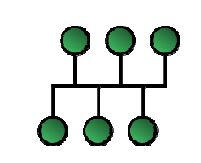
\includegraphics[width=1\textwidth]{figures/bus.JPG}}
  	\caption{Topologi bus.}
  	\label{bus}
  	\end{figure}
    Gambar ini \ref{bus} adalah topologi bus,berdasarkan artikel yudianto Topologi bus merupakan topologi yang banyak digunakan pada masa penggunaan kabel sepaksi menjamur\cite{yudianto2007jaringan}. Dengan menggunakan T-Connector(dengan terminator 50ohm pada ujung network), maka komputer atau perangkat jaringan lainnya bisa dengan mudah dihubungkan satu sama lain.
  Kesulitan utama dari penggunaan kabel sepaksi adalah sulit uuntuk mengukur apakah kabel sepakksi yang di gunakan benar-benar matching atau tidak. Karena kalau tidak sungguh-sungguh diukur secara benar akan merusak NIC yang digunakan dan kinerja jaringan menjadi terhambat, tidak mencapai kemampuan maksimalnya. Topologi ini juga sering digunakan pada jaringan dengan basis FO.
  \subsubsection{Topologi Star}
    \ref{star}
    \begin{figure}[ht]
    \centerline{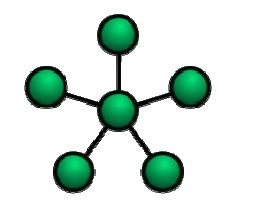
\includegraphics[width=1\textwidth]{figures/star.JPG}}
    \caption{Topologi star.}
    \label{star}
    \end{figure}
    Gambar ini \ref{star} adalah topologi star,berdasarkan artikel tudianto Topologi bintang merupakan bentuk topologi jaringan yang berupa konvergensi dari node tengah ke setiap node atau pengguna\cite{yudianto2007jaringan}. Topologi jaringan bintang termasuk topologi jaringan dengan biaya menengah.
  \subsubsection{Topologi Ring}
    \ref{ring}
    \begin{figure}[ht]
    \centerline{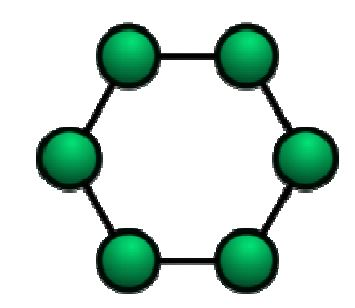
\includegraphics[width=1\textwidth]{figures/ring.JPG}}
    \caption{Topologi ring.}
    \label{ring}
    \end{figure}
    Gambar ini \ref{ring} adalah topologi ring/cincin,berdasarkan artikel yudianto Topologi cincin adalah topologi jaringan berbentuk rangkaian titik yang masing-masing terhubung ke dua titik lainnya, sedemikian sehingga membentuk jalur melingkar membentuk cincin\cite{yudianto2007jaringan}. Pada Topologi cincin,masing - masing titik/node berfungsi sebagai repeater yang akan memperkuat sinyal disepanjang sirkulasinya, artinya masing - masing perangkat saling bekerjasama untuk menerima sinyal dari perangkat sebelumnya kemudian meneruskannya pada perangkat sesudahnya, proses menerima dan meneruskan sinyal data ini dibantu oleh TOKEN. TOKEN berisi informasi bersamaan dengan data yang berasal dari komputer sumber, token kemudian akan melewati titik/node dan akan memeriksa apakah informasi data tersebut digunakan oleh titik/node yang bersangkutan, jika ya maka token akan memberikan data yang diminta oleh node untuk kemudian kembali berjalan ke titik/node berikutnya dalam jaringan. Jika tidak maka token akan melewati titik/node sambil membawa data menuju ke titik/node berikutnya. proses ini akan terus berlangsung hingga sinyal data mencapai tujuannya.
  \subsubsection{Topologi Mesh}
    \ref{mesh}
    \begin{figure}[ht]
    \centerline{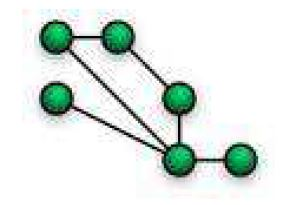
\includegraphics[width=1\textwidth]{figures/mesh.JPG}}
    \caption{Topologi mesh.}
    \label{mesh}
    \end{figure}
    Gambar ini \ref{mesh} adalah topologi mesh, berdasarkan artikel dari yudianto Topologi mesh adalah suatu bentuk hubungan antar perangkat dimana setiap perangkat terhubung secara langsung ke perangkat lainnya yang ada di dalam jaringan\cite{yudianto2007jaringan}. Akibatnya, dalam topologi mesh setiap perangkat dapat berkomunikasi langsung dengan perangkat yang dituju (dedicated links). Dengan demikian maksimal banyaknya koneksi antar perangkat pada jaringan bertopologi mesh ini dapat dihitung yaitu sebanyak \begin{equation}n(n-1)/2\end{equation}. 
    Selain itu karena setiap perangkat dapat terhubung dengan perangkat lainnya yang ada di dalam jaringan maka setiap perangkat harus memiliki sebanyak n-1 Port Input/Output (I/O ports).Berdasarkan pemahaman di atas, dapat dicontohkan bahwa apabila sebanyak 5(lima) komputer akan dihubungkan dalam bentuk topologi mesh maka agar seluruh koneksi antar komputer dapat berfungsi optimal, diperlukan kabel koneksi sebanyak \begin{verbatim}5(5-1)/2 = 10 \end{verbatim} kabel koneksi, dan masing-masing komputer harus memiliki port I/O sebanyak 5-1 = 4 port.
  \subsubsection{Topologi Tree}
    \ref{tree}
    \begin{figure}[ht]
    \centerline{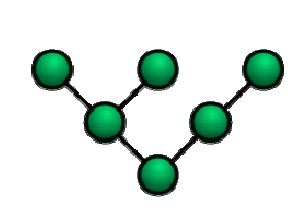
\includegraphics[width=1\textwidth]{figures/tree.JPG}}
    \caption{Topologi tree.}
    \label{tree}
    \end{figure}
    Gambar ini \ref{tree} adalah topologi tree, berdasarkan artikel dari yudianto Topologi Pohon adalah kombinasi karakteristik antara topologi bintang dan topologi bus\cite{yudianto2007jaringan}. Topologi ini terdiri atas kumpulan topologi bintang yang dihubungkan dalam satu topologi bus sebagai jalur tulang punggung atau backbone. Komputer-komputer dihubungkan ke hub, sedangkan hub lain di hubungkan sebagai jalur tulang punggung.Topologi jaringan ini disebut juga sebagai topologi jaringan bertingkat. Topologi ini biasanya digunakan untuk interkoneksi antar sentral dengan hirarki yang berbeda. Untuk hirarki yang lebih rendah digambarkan pada lokasi yang rendah dan semakin keatas mempunyai hirarki semakin tinggi. Topologi jaringan jenis ini cocok digunakan pada sistem jaringan komputer.Pada jaringan pohon, terdapat beberapa tingkatan simpul atau node.Pusat atau simpul yang lebih tinggi tingkatannya, dapat mengatur simpul lain yang lebih rendah tingkatannya. Data yang dikirim perlu melalui simpul pusat terlebih dahulu. Misalnya untuk bergerak dari komputer dengan node-3 kekomputer node-7 seperti halnya pada gambar, data yang ada harus melewati node-3, 5 dan node-6 sebelum berakhir pada node-7.
  \subsubsection{Topologi Linier}
    \ref{linier}
    \begin{figure}[ht]
    \centerline{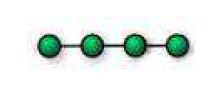
\includegraphics[width=1\textwidth]{figures/linier.JPG}}
    \caption{Topologi linier.}
    \label{linier}
    \end{figure}
    Gambar ini \ref{linier} adalah topologi linier, Topologi ini biasa disebut dengan topologi bus beruntut, tata letak ini termasuk tata letak umum.

\begin{table}[ht]
	\caption{Kekurangan dan Kelebihan}
	\centering
	\begin{tabular}{cccc}
		\hline
		No&Kelebihan&Kekurangan&\\
		\hline
		.1&Hemat kabel&Deteksi dan isolasi kesalahan sangat kecil&\\
		.2&Tata letak kabel sederhana&Kepadatan lalu lintas tinggi&\\
		.3&Mudah dikembangkan& Keamanan dta kurang terjamin&\\
		\hline
	\end{tabular}
\end{table}

\section{Alat-alat jaringan}
Macam-macam alat jaringan antara lain :
  \subsection{ROUTER}
    Router adalah sebuah alat yang mengirimkan paket data melalui sebuah jaringan atau Internet menuju tujuannya, alat ini sangatlah penting untuk meneruskan jaringan satu ke jaringan lainnya yang berbeda kelas/subnet/ip. melalui sebuah proses yang dikenal sebagai routing. Proses routing terjadi pada lapisan 3 (Lapisan jaringan seperti Internet Protocol) dari stack protokol tujuh-lapis OSI.
  Router berfungsi sebagai penghubung antar dua atau lebih jaringan untuk meneruskan data dari satu jaringan ke jaringan lainnya. Router berbeda dengan switch. Switch merupakan penghubung beberapa alat untuk membentuk suatu Local Area Network (LAN).
  \subsection{SWITCH}
    Switch adalah perangkat jaringan komputer yang bekerja di OSI Layer 2, Data Link Layer. Switch kerjanya sebagai penyambung atau concentrator dalam Jaringan komputer. Switch mengenal MAC Adressing shingga dia bisa memilah paket data mana yang akan di teruskan/dilanjutkan ke mana.
\subsection{ACCESS POINT}
    Access point adalah perangkat yang digunakan sebagai pembuat koneksi wireless pada jaringan komputer. Fungsi Access point diantaranya: Sebagai perangkat jaringan yang berfungsi membuat jaringan komputer tanpa kabel, atau biasa disebut WI-FI (Wireless Fidelity)
  Belajar Network Programming pada python, melalui fungsi-fungsi TCP/IP, SOCKET, dll.

\section{Latihan Jaringan pada python}
Pada latihan ini, kita akan mencoba mengirim data dari server menuju klien dengan menggunakan Socket pada python.
\subsection{server.py}
Penjelasan fungsi-fungsi tsb akan dijelaskan dibawah ini:
\begin{enumerate}
 \item socket.socket(): Membuat socket baru menggunakan alamat yang sudah ada, tipe socket, dan nomor protocol.
 \item socket.bind(address): Menyalin/mengikat socket ke alamat yang ada.
 \item socket.listen(backlog): Menunggu koneksi yang sudah dibuat dari socket tersebut. backlog merupakan sebuah argumen yang menyatakan batas maximal nomor antrian koneksi dan paling tidak sampai dengan 0; nilai maximum tergantung dari sistem(biasanya 5), dan nilai minimumnya harus mencapai 0.
 \item socket.accept(): Nilai yang dikembalikan atau diberikan adalah sepasang(conn, address) dimana conn adalah socket baru yaitu sebuah objek yang biasa digunakan untuk mengirim dan menerima data dari koneksi tersebut dan address adalah alamat yang terikat ke socket pada akhir koneksi.
 \item socket.send(bytes[, flags]): Mengiri data ke socket. Socket harus terkoneksi oleh remote Socket. mengembalikan angkat dari bytes yang terkirim. Aplikasi yang bertugas untuk mengecek semua data harus terkirim; hanya jika data ditransimisikan, aplikasi membutuhkan usaha untuk mengirimkan data yang tersisa.
 \item socket.close(): Menandakan bahwa socket telah ditutup. semua dari operasi-operasi pada objek socket akan gagal. Remote End tidak akan menerima data lagi (sampai data telah dibersihkan). Socket-socket secara otomatis tertutup ketika dilakukan garbage-collected, tetapi lebih baik untuk close() mereka secara eksplisit.
\end{enumerate}
Sebelumnya pesan diatas tidak akan muncul sebelum kita menjalankan script client.py pada tab terminal lain.
maka setiap kali kita menjalankan script client.py akan terus mengirimkan pesan kepada server maupun client.

contoh networking:
\begin{verbatim}
192.168.0.0/24 subnet mask 255.255.255.0, 256 IP rumus-nya

(jumlah IP network diatas / 2) + (subnetmask diatasnya)= subnetmask yang digunakan

(256/2) + n = 128, jadi subnet mask buat 128 ip adalah 255.255.255.128
(128/2) + 128 = 192, jadi subnetmask buat 64 ip adalah 255.255.255.192
(64/2) + 192 = 224, jadi subnet mask buat 32 ip adalah 255.255.255.224
(32/2) + 224 = 240, jadi subnet mask buat 16 ip adalah 255.255.255.240
(16/2) + 240 = 248, jadi subnet mask buat 8 ip adalah 255.255.255.248
(8/2) + 248 = 252, jadi subnet mask buat 4 ip adalah 255.255.255.252
(4/2) + 252 = 254, jadi subnet mask buat 2 ip adalah 255.255.255.254
(2/2) + 254 = 255, jadi subnet mask buat 1 ip adalah 255.255.255.255
\end{verbatim}